% Options for packages loaded elsewhere
\PassOptionsToPackage{unicode}{hyperref}
\PassOptionsToPackage{hyphens}{url}
\PassOptionsToPackage{dvipsnames,svgnames,x11names}{xcolor}
%
\documentclass[
  letterpaper,
  DIV=11,
  numbers=noendperiod]{scrartcl}

\usepackage{amsmath,amssymb}
\usepackage{lmodern}
\usepackage{iftex}
\ifPDFTeX
  \usepackage[T1]{fontenc}
  \usepackage[utf8]{inputenc}
  \usepackage{textcomp} % provide euro and other symbols
\else % if luatex or xetex
  \usepackage{unicode-math}
  \defaultfontfeatures{Scale=MatchLowercase}
  \defaultfontfeatures[\rmfamily]{Ligatures=TeX,Scale=1}
\fi
% Use upquote if available, for straight quotes in verbatim environments
\IfFileExists{upquote.sty}{\usepackage{upquote}}{}
\IfFileExists{microtype.sty}{% use microtype if available
  \usepackage[]{microtype}
  \UseMicrotypeSet[protrusion]{basicmath} % disable protrusion for tt fonts
}{}
\makeatletter
\@ifundefined{KOMAClassName}{% if non-KOMA class
  \IfFileExists{parskip.sty}{%
    \usepackage{parskip}
  }{% else
    \setlength{\parindent}{0pt}
    \setlength{\parskip}{6pt plus 2pt minus 1pt}}
}{% if KOMA class
  \KOMAoptions{parskip=half}}
\makeatother
\usepackage{xcolor}
\setlength{\emergencystretch}{3em} % prevent overfull lines
\setcounter{secnumdepth}{-\maxdimen} % remove section numbering
% Make \paragraph and \subparagraph free-standing
\ifx\paragraph\undefined\else
  \let\oldparagraph\paragraph
  \renewcommand{\paragraph}[1]{\oldparagraph{#1}\mbox{}}
\fi
\ifx\subparagraph\undefined\else
  \let\oldsubparagraph\subparagraph
  \renewcommand{\subparagraph}[1]{\oldsubparagraph{#1}\mbox{}}
\fi

\usepackage{color}
\usepackage{fancyvrb}
\newcommand{\VerbBar}{|}
\newcommand{\VERB}{\Verb[commandchars=\\\{\}]}
\DefineVerbatimEnvironment{Highlighting}{Verbatim}{commandchars=\\\{\}}
% Add ',fontsize=\small' for more characters per line
\usepackage{framed}
\definecolor{shadecolor}{RGB}{241,243,245}
\newenvironment{Shaded}{\begin{snugshade}}{\end{snugshade}}
\newcommand{\AlertTok}[1]{\textcolor[rgb]{0.68,0.00,0.00}{#1}}
\newcommand{\AnnotationTok}[1]{\textcolor[rgb]{0.37,0.37,0.37}{#1}}
\newcommand{\AttributeTok}[1]{\textcolor[rgb]{0.40,0.45,0.13}{#1}}
\newcommand{\BaseNTok}[1]{\textcolor[rgb]{0.68,0.00,0.00}{#1}}
\newcommand{\BuiltInTok}[1]{\textcolor[rgb]{0.00,0.23,0.31}{#1}}
\newcommand{\CharTok}[1]{\textcolor[rgb]{0.13,0.47,0.30}{#1}}
\newcommand{\CommentTok}[1]{\textcolor[rgb]{0.37,0.37,0.37}{#1}}
\newcommand{\CommentVarTok}[1]{\textcolor[rgb]{0.37,0.37,0.37}{\textit{#1}}}
\newcommand{\ConstantTok}[1]{\textcolor[rgb]{0.56,0.35,0.01}{#1}}
\newcommand{\ControlFlowTok}[1]{\textcolor[rgb]{0.00,0.23,0.31}{#1}}
\newcommand{\DataTypeTok}[1]{\textcolor[rgb]{0.68,0.00,0.00}{#1}}
\newcommand{\DecValTok}[1]{\textcolor[rgb]{0.68,0.00,0.00}{#1}}
\newcommand{\DocumentationTok}[1]{\textcolor[rgb]{0.37,0.37,0.37}{\textit{#1}}}
\newcommand{\ErrorTok}[1]{\textcolor[rgb]{0.68,0.00,0.00}{#1}}
\newcommand{\ExtensionTok}[1]{\textcolor[rgb]{0.00,0.23,0.31}{#1}}
\newcommand{\FloatTok}[1]{\textcolor[rgb]{0.68,0.00,0.00}{#1}}
\newcommand{\FunctionTok}[1]{\textcolor[rgb]{0.28,0.35,0.67}{#1}}
\newcommand{\ImportTok}[1]{\textcolor[rgb]{0.00,0.46,0.62}{#1}}
\newcommand{\InformationTok}[1]{\textcolor[rgb]{0.37,0.37,0.37}{#1}}
\newcommand{\KeywordTok}[1]{\textcolor[rgb]{0.00,0.23,0.31}{#1}}
\newcommand{\NormalTok}[1]{\textcolor[rgb]{0.00,0.23,0.31}{#1}}
\newcommand{\OperatorTok}[1]{\textcolor[rgb]{0.37,0.37,0.37}{#1}}
\newcommand{\OtherTok}[1]{\textcolor[rgb]{0.00,0.23,0.31}{#1}}
\newcommand{\PreprocessorTok}[1]{\textcolor[rgb]{0.68,0.00,0.00}{#1}}
\newcommand{\RegionMarkerTok}[1]{\textcolor[rgb]{0.00,0.23,0.31}{#1}}
\newcommand{\SpecialCharTok}[1]{\textcolor[rgb]{0.37,0.37,0.37}{#1}}
\newcommand{\SpecialStringTok}[1]{\textcolor[rgb]{0.13,0.47,0.30}{#1}}
\newcommand{\StringTok}[1]{\textcolor[rgb]{0.13,0.47,0.30}{#1}}
\newcommand{\VariableTok}[1]{\textcolor[rgb]{0.07,0.07,0.07}{#1}}
\newcommand{\VerbatimStringTok}[1]{\textcolor[rgb]{0.13,0.47,0.30}{#1}}
\newcommand{\WarningTok}[1]{\textcolor[rgb]{0.37,0.37,0.37}{\textit{#1}}}

\providecommand{\tightlist}{%
  \setlength{\itemsep}{0pt}\setlength{\parskip}{0pt}}\usepackage{longtable,booktabs,array}
\usepackage{calc} % for calculating minipage widths
% Correct order of tables after \paragraph or \subparagraph
\usepackage{etoolbox}
\makeatletter
\patchcmd\longtable{\par}{\if@noskipsec\mbox{}\fi\par}{}{}
\makeatother
% Allow footnotes in longtable head/foot
\IfFileExists{footnotehyper.sty}{\usepackage{footnotehyper}}{\usepackage{footnote}}
\makesavenoteenv{longtable}
\usepackage{graphicx}
\makeatletter
\def\maxwidth{\ifdim\Gin@nat@width>\linewidth\linewidth\else\Gin@nat@width\fi}
\def\maxheight{\ifdim\Gin@nat@height>\textheight\textheight\else\Gin@nat@height\fi}
\makeatother
% Scale images if necessary, so that they will not overflow the page
% margins by default, and it is still possible to overwrite the defaults
% using explicit options in \includegraphics[width, height, ...]{}
\setkeys{Gin}{width=\maxwidth,height=\maxheight,keepaspectratio}
% Set default figure placement to htbp
\makeatletter
\def\fps@figure{htbp}
\makeatother

\usepackage{booktabs}
\usepackage{longtable}
\usepackage{array}
\usepackage{multirow}
\usepackage{wrapfig}
\usepackage{float}
\usepackage{colortbl}
\usepackage{pdflscape}
\usepackage{tabu}
\usepackage{threeparttable}
\usepackage{threeparttablex}
\usepackage[normalem]{ulem}
\usepackage{makecell}
\usepackage{xcolor}
\usepackage{siunitx}

  \newcolumntype{d}{S[
    input-open-uncertainty=,
    input-close-uncertainty=,
    parse-numbers = false,
    table-align-text-pre=false,
    table-align-text-post=false
  ]}
  
\KOMAoption{captions}{tableheading}
\makeatletter
\@ifpackageloaded{tcolorbox}{}{\usepackage[many]{tcolorbox}}
\@ifpackageloaded{fontawesome5}{}{\usepackage{fontawesome5}}
\definecolor{quarto-callout-color}{HTML}{909090}
\definecolor{quarto-callout-note-color}{HTML}{0758E5}
\definecolor{quarto-callout-important-color}{HTML}{CC1914}
\definecolor{quarto-callout-warning-color}{HTML}{EB9113}
\definecolor{quarto-callout-tip-color}{HTML}{00A047}
\definecolor{quarto-callout-caution-color}{HTML}{FC5300}
\definecolor{quarto-callout-color-frame}{HTML}{acacac}
\definecolor{quarto-callout-note-color-frame}{HTML}{4582ec}
\definecolor{quarto-callout-important-color-frame}{HTML}{d9534f}
\definecolor{quarto-callout-warning-color-frame}{HTML}{f0ad4e}
\definecolor{quarto-callout-tip-color-frame}{HTML}{02b875}
\definecolor{quarto-callout-caution-color-frame}{HTML}{fd7e14}
\makeatother
\makeatletter
\makeatother
\makeatletter
\makeatother
\makeatletter
\@ifpackageloaded{caption}{}{\usepackage{caption}}
\AtBeginDocument{%
\ifdefined\contentsname
  \renewcommand*\contentsname{Table of contents}
\else
  \newcommand\contentsname{Table of contents}
\fi
\ifdefined\listfigurename
  \renewcommand*\listfigurename{List of Figures}
\else
  \newcommand\listfigurename{List of Figures}
\fi
\ifdefined\listtablename
  \renewcommand*\listtablename{List of Tables}
\else
  \newcommand\listtablename{List of Tables}
\fi
\ifdefined\figurename
  \renewcommand*\figurename{Figure}
\else
  \newcommand\figurename{Figure}
\fi
\ifdefined\tablename
  \renewcommand*\tablename{Table}
\else
  \newcommand\tablename{Table}
\fi
}
\@ifpackageloaded{float}{}{\usepackage{float}}
\floatstyle{ruled}
\@ifundefined{c@chapter}{\newfloat{codelisting}{h}{lop}}{\newfloat{codelisting}{h}{lop}[chapter]}
\floatname{codelisting}{Listing}
\newcommand*\listoflistings{\listof{codelisting}{List of Listings}}
\makeatother
\makeatletter
\@ifpackageloaded{caption}{}{\usepackage{caption}}
\@ifpackageloaded{subcaption}{}{\usepackage{subcaption}}
\makeatother
\makeatletter
\@ifpackageloaded{tcolorbox}{}{\usepackage[many]{tcolorbox}}
\makeatother
\makeatletter
\@ifundefined{shadecolor}{\definecolor{shadecolor}{rgb}{.97, .97, .97}}
\makeatother
\makeatletter
\makeatother
\ifLuaTeX
  \usepackage{selnolig}  % disable illegal ligatures
\fi
\IfFileExists{bookmark.sty}{\usepackage{bookmark}}{\usepackage{hyperref}}
\IfFileExists{xurl.sty}{\usepackage{xurl}}{} % add URL line breaks if available
\urlstyle{same} % disable monospaced font for URLs
\hypersetup{
  pdftitle={Problem Set 8},
  colorlinks=true,
  linkcolor={blue},
  filecolor={Maroon},
  citecolor={Blue},
  urlcolor={Blue},
  pdfcreator={LaTeX via pandoc}}

\title{Problem Set 8}
\usepackage{etoolbox}
\makeatletter
\providecommand{\subtitle}[1]{% add subtitle to \maketitle
  \apptocmd{\@title}{\par {\large #1 \par}}{}{}
}
\makeatother
\subtitle{Due date: 20 November}
\author{}
\date{}

\begin{document}
\maketitle
\ifdefined\Shaded\renewenvironment{Shaded}{\begin{tcolorbox}[boxrule=0pt, interior hidden, frame hidden, borderline west={3pt}{0pt}{shadecolor}, enhanced, sharp corners, breakable]}{\end{tcolorbox}}\fi

\renewcommand*\contentsname{Table of contents}
{
\hypersetup{linkcolor=}
\setcounter{tocdepth}{3}
\tableofcontents
}
Please upload your completed assignment to the ELMs course site (under
the assignments menu). Remember to include an annotated script file for
all work with R and show your math for all other problems (if
applicable, or necessary). Please also upload your completed assignment
to the Github repository that you have shared with us. \emph{We should
be able to run your script with no errors.}

\textbf{Total points: 30}

\hypertarget{question-1}{%
\subsection{Question 1}\label{question-1}}

\emph{Points: 5}

For the following regression equation,
\(\hat{Y} = 8.5 + 6x + \epsilon\), the standard error for \(\beta_0\) is
2.5, the standard error for \(\beta_1\) is 3.5, and the sample size is
2000. Find the t-statistic, 95\% confidence interval, and p-value (using
a two-tailed test) for \(\beta_1\).

Is \(\beta_1\) statistically significant at the 0.05-level with a
two-tailed test? Why or why not?

t-statistic:

\(t = \frac{6-0}{3.5} = 1.71\)

The 95\% CI:

Upper bound: 6 + 1.961 x 3.5 = 12.86

Lower bound: 6 -1.961 x 3.5 = -0.86

The 95\% confidence interval for \(\beta_1\)\hspace{0pt} is
approximately from -0.86 to 12.86. The interval suggests that, with 95\%
confidence, we can say the true value of
\(\beta_1\)\hspace{0pt}\hspace{0pt} lies somewhere within this range.

P-value:\\
With a t-statistic of 1.71 and 1998 degrees of freedom, we get a p-value
of .087

β1\hspace{0pt} is not statistically significant at the 0.05 level based
on the t-statistic, p-value, and confidence interval, meaning we don't
have enough evidence to say that \(\beta_1\)\hspace{0pt} is different
from 0.

\hypertarget{question-2}{%
\subsection{Question 2}\label{question-2}}

\emph{Points: 5}

Suppose you estimate an OLS regression and retrieve a \(R^2\) value of
0.45. If the Total Sum of Squares (TSS) from that regression equals
4,700, what is the value for the Residual Sum of Squares (RSS)?

\(RSS = 4700\times(1-0.45)= 2585\)

This tells us that the total variance in the DV, the models residuals
account for 2585 units.

\hypertarget{question-3}{%
\subsection{Question 3}\label{question-3}}

\emph{Points: 5}

Suppose you estimate a bivariate regression with a sample size of 102
and obtain a regression coefficient (\(\beta_1\)) of 5.0. What is the
largest standard error that \(\beta_1\) could have and still be
statistically significant (i.e., reject the null hypothesis of no
relationship) at the 0.05 level with a one-tailed test?

\(SE(β1​) = \frac{5.0}{1.66} = 3.01\)

The largest standard error for \(\beta_1\) that still allows for
statistical significance at the 0.05 level about 3.01. This means if the
actual SE of \(\beta_1\) \hspace{0pt} is less than or equal to 3.01, the
coefficient is statistically significant at the 5\% level, which will
reject the null.

\hypertarget{question-4}{%
\subsection{Question 4}\label{question-4}}

\emph{Points: 5}

Using the \texttt{states} dataset from the \texttt{poliscidata} package,
produce a scatterplot of the variables \texttt{romney2012} and
\texttt{hispanic10} (with \texttt{romney2012} as the dependent variable
on the y-axis). Fit a regression line to the scatterplot. Describe the
scatterplot and include a copy of it. Note any suspected outliers, if
any (a visual inspection will suffice for this question).

\begin{tcolorbox}[enhanced jigsaw, coltitle=black, colframe=quarto-callout-note-color-frame, breakable, bottomrule=.15mm, bottomtitle=1mm, colback=white, left=2mm, toptitle=1mm, arc=.35mm, title=\textcolor{quarto-callout-note-color}{\faInfo}\hspace{0.5em}{Note}, colbacktitle=quarto-callout-note-color!10!white, titlerule=0mm, rightrule=.15mm, toprule=.15mm, leftrule=.75mm, opacitybacktitle=0.6, opacityback=0]

The variable \texttt{romney2012} measures the percentage of the state's
vote that Mitt Romney received in the 2012 presidential election, and
\texttt{hispanic10} indicates the percentage of the state's population
that identified as Hispanic in 2010.

\end{tcolorbox}

\begin{Shaded}
\begin{Highlighting}[]
\FunctionTok{library}\NormalTok{(poliscidata)}
\end{Highlighting}
\end{Shaded}

\begin{verbatim}
Registered S3 method overwritten by 'gdata':
  method         from  
  reorder.factor gplots
\end{verbatim}

\begin{Shaded}
\begin{Highlighting}[]
\FunctionTok{library}\NormalTok{(modelsummary)}
\FunctionTok{library}\NormalTok{(tidyverse)}
\end{Highlighting}
\end{Shaded}

\begin{verbatim}
-- Attaching core tidyverse packages ------------------------ tidyverse 2.0.0 --
v dplyr     1.1.3     v readr     2.1.4
v forcats   1.0.0     v stringr   1.5.0
v ggplot2   3.4.3     v tibble    3.2.1
v lubridate 1.9.2     v tidyr     1.3.0
v purrr     1.0.1     
\end{verbatim}

\begin{verbatim}
-- Conflicts ------------------------------------------ tidyverse_conflicts() --
x dplyr::filter() masks stats::filter()
x dplyr::lag()    masks stats::lag()
i Use the ]8;;http://conflicted.r-lib.org/conflicted package]8;; to force all conflicts to become errors
\end{verbatim}

\begin{Shaded}
\begin{Highlighting}[]
\FunctionTok{library}\NormalTok{(ggplot2)}
\FunctionTok{ggplot}\NormalTok{(states, }\FunctionTok{aes}\NormalTok{(}\AttributeTok{x =}\NormalTok{ hispanic10, }\AttributeTok{y =}\NormalTok{ romney2012))}\SpecialCharTok{+}
  \FunctionTok{geom\_point}\NormalTok{()}\SpecialCharTok{+}
  \FunctionTok{geom\_smooth}\NormalTok{(}\AttributeTok{method =}\NormalTok{ lm, }\AttributeTok{se =}\NormalTok{ F)}\SpecialCharTok{+}
  \FunctionTok{theme\_classic}\NormalTok{()}
\end{Highlighting}
\end{Shaded}

\begin{verbatim}
`geom_smooth()` using formula = 'y ~ x'
\end{verbatim}

\begin{figure}[H]

{\centering 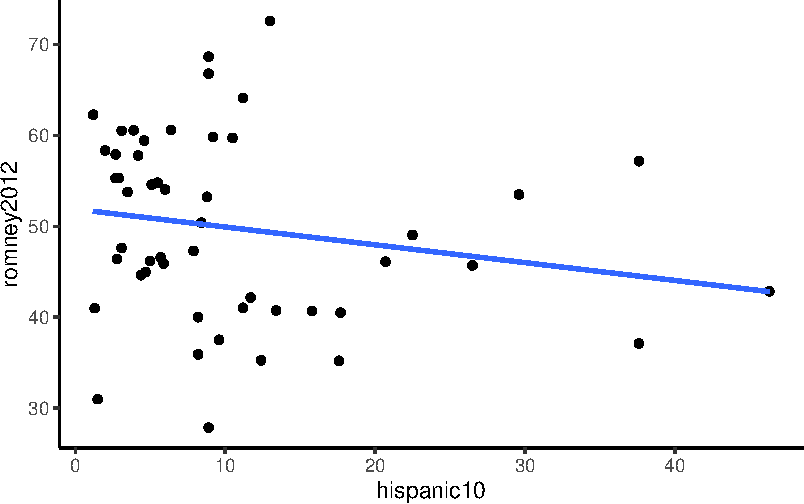
\includegraphics{problem_set_8_files/figure-pdf/unnamed-chunk-1-1.pdf}

}

\end{figure}

\begin{Shaded}
\begin{Highlighting}[]
\FunctionTok{cor}\NormalTok{(states}\SpecialCharTok{$}\NormalTok{romney2012, states}\SpecialCharTok{$}\NormalTok{hispanic10)}
\end{Highlighting}
\end{Shaded}

\begin{verbatim}
[1] -0.1918332
\end{verbatim}

This scatterplot shows a negative trend, as shown by the downward slope
line. As the percentage of the Hispanic population increases, the
percentage of votes for Mitt Romney decreases. The correlation for this
scatter is -0.19

\hypertarget{question-5}{%
\subsection{Question 5}\label{question-5}}

\emph{Points: 10}

Estimate a bivariate regression with \texttt{romney2012} as the
dependent variable and \texttt{hispanic10} as the independent variable
and report the results in a professionally formatted table. In as much
detail as possible, describe (and interpret) the regression results.

\begin{Shaded}
\begin{Highlighting}[]
\NormalTok{model }\OtherTok{\textless{}{-}} \FunctionTok{lm}\NormalTok{(romney2012 }\SpecialCharTok{\textasciitilde{}}\NormalTok{ hispanic10, }\AttributeTok{data =}\NormalTok{ states)}
\FunctionTok{modelsummary}\NormalTok{(model,}
             \AttributeTok{coef\_rename =} \FunctionTok{c}\NormalTok{(}\StringTok{"hispanic10"} \OtherTok{=} \StringTok{"Hispanic pop in a state"}\NormalTok{),}
             \AttributeTok{statistic =} \FunctionTok{c}\NormalTok{(}\StringTok{"conf.int"}\NormalTok{,}\StringTok{"p.value"}\NormalTok{))}
\end{Highlighting}
\end{Shaded}

\begin{table}
\centering
\begin{tabular}[t]{lc}
\toprule
  & (1)\\
\midrule
(Intercept) & \num{51.877}\\
 & {}[\num{47.655}, \num{56.098}]\\
 & (\num{<0.001})\\
Hispanic pop in a state & \num{-0.196}\\
 & {}[\num{-0.487}, \num{0.095}]\\
 & (\num{0.182})\\
\midrule
Num.Obs. & \num{50}\\
R2 & \num{0.037}\\
R2 Adj. & \num{0.017}\\
AIC & \num{377.3}\\
BIC & \num{383.0}\\
Log.Lik. & \num{-185.642}\\
F & \num{1.834}\\
RMSE & \num{9.91}\\
\bottomrule
\end{tabular}
\end{table}

Our regression result shows that the intercept is 51.87, with a 95\%
confident interval of between 47.65 and 56.09, this suggests that if the
percentage of the hispanic population were zero the predicted outcome
would be 51.87. because out interval does not contain zero its indicate
that the intercept is statistically significant. The coefficint in out
model shows -0.196 meaning that for every one percentage point increase
in the Hispanic population within a state, the dependent variable is
expected to decrease by 0.196 percentage points, holding all else
constant. Our model shows an R-squared of 0.037, which means that
approximately 3.7\% of the variance in the dependent variable is
explained by the x variable. This is a very low value, indicating that
the model does not explain much of the variance. Similarly, the adjusted
R-squared value is 0.017,which further confirms that the model explains
very little of the variance in the dependent variable. Finally, the
p-value associated with the coefficient is 0.182.



\end{document}
